\chapter{Marco Teórico Contextual}

\section{Marco Teórico Contextual}
Para contextualizar adecuadamente el presente trabajo de tesis dentro del marco teórico, es necesario abordar el origen del algoritmo criptográfico estándar César, así como su evolución y aplicaciones a lo largo del tiempo. Asimismo, se explorarán las condiciones en las que surgieron los servicios y mecanismos de seguridad informática, y las formas en que estos han sido implementados en distintos entornos. Este análisis permite delimitar la problemática que se busca atender mediante la propuesta de implementación en hardware presentada en esta investigación. En consecuencia, se realiza una revisión del estado del arte en la disciplina, con especial énfasis en los sistemas embebidos que incorporan mecanismos de seguridad.

A través de esta revisión se busca comprender las bases que fundamentan el diseño de soluciones criptográficas en plataformas reconfigurables, como las FPGAs, y su relevancia en escenarios donde la protección de la información es crítica. Este marco teórico sienta las bases para el desarrollo metodológico y experimental abordado en los siguientes capítulos.

\section{Fundamentos de la Criptografía clasica}
La criptografía es la ciencia y arte de proteger la información mediante técnicas que transforman datos legibles (texto plano) en datos ininteligibles (texto cifrado), de modo que sólo las personas autorizadas puedan acceder a su contenido (Stallings, 2017). A lo largo de la historia, la criptografía ha evolucionado desde métodos simples de sustitución y transposición hasta complejos algoritmos basados en teoría matemática, álgebra moderna y teoría de números.

Los métodos clásicos, aunque hoy son inseguros frente a los ataques modernos, permiten comprender los conceptos fundamentales sobre el uso de claves, cifrado simétrico y análisis criptográfico. Uno de los algoritmos más representativos de la criptografía clásica es el cifrado César, también conocido como cifrado por desplazamiento.

\section{El Cifrado César: Origen Histórico}
El cifrado César recibe su nombre de Julio César, quien lo empleaba para cifrar mensajes militares. Según registros históricos, César utilizaba un desplazamiento de tres posiciones para codificar sus mensajes (Kahn, 1996). Aunque su simplicidad hoy lo convierte en un cifrado trivial, en su época ofrecía una protección básica frente a lectores no entrenados o no alfabetizados.

Este cifrado pertenece a la familia de los cifrados monoalfabéticos por sustitución, donde cada letra del alfabeto es reemplazada por otra, según una regla fija determinada por una clave de desplazamiento.

\section{Funcionamiento del Algoritmo}

Desde un punto de vista matemátoco, el cifrado César puede representarse mediante la siguiente función:

\centerline{\(C(x) = ( x + k ) mod n \)}

Donde:

\begin{itemize}
\item \(C(x)\) es el carácter cifrado.
\item \(x\) es el índice del carácter en el alfabeto \( A = 0, B = 1, ...., Z = 25\)
\item \(k \) es la clave de desplazamiento.
\item \(n\) el es número total de caracteres del alfabeto, usualmente  \(n = 26 \) en el alfabeto latino.
\end{itemize}

El descifrado consiste en aplicar la operación inversa 

\centerline{\(P(x) = ( x - k ) mod n \)}

Por ejemplo, si se cifra la palabra \textbf{\textit{''HOLA''}} con un desplazamiento de \(k = 3\) se obtiene \textbf{\textit{''KROD''}} . Para descifrar, se aplica el desplazamiento inverso. 

\section{Seguridad y Vulnerabilidades}

El cifrado César es vulnerable a varios tipos de ataques criptográficos:

\begin{itemize}
\item Ataque por fuerza bruta: Dado que existen solamente 25 posibles claves (excluyendo el desplazamiento nulo), un atacante puede probar todas las combinaciones en poco tiempo.
\item Análisis de frecuencia: Cada idioma tiene una distribución característica de letras. En español, por   las letras ''E'', ''A'' y ''O'' son las más comunes. Si se cifra un texto suficientemente largo, estas frecuencias se preservan, permitiendo identificar el desplazamiento utilizado.
\end{itemize}

Estas debilidades lo hacen inapropiado para cualquier uso moderno que requiera confidencialidad real, pero útil como herramienta de desarrollo.

\section{Utilidad en el Diseño de Sistemas Criptográficos}
A pesar de sus limitaciones, el cifrado César es frecuentemente utilizado en el diseño de sistemas criptográficos hardware/software con fines educativos y experimentales. Su estructura simple lo convierte en una opción ideal para:

\begin{itemize}
\item Introducir técnicas de procesamiento secuencial de datos.
\item Implementar máquinas de estados finitos para codificación y decodificación.
\item Evaluar el consumo de recursos lógicos y tiempos de propagación en plataformas como FPGAs.
\item Comparar el comportamiento de cifrados más complejos respecto a algoritmos básicos en entornos de bajo nivel (VHDL, Verilog).
\end{itemize}

En proyectos de diseño digital con arquitectura RTL (Register Transfer Level), el cifrado César se utiliza como caso de estudio para optimizar operaciones de desplazamiento modular, codificación de caracteres ASCII y generación de claves.



\chapter{Antecedentes System Verilog}

\section{Evolución del diseño digital y el surgimiento de SystemVerilog}
El desarrollo del diseño digital ha experimentado transformaciones significativas desde sus inicios, comenzando con el prototipado físico mediante placas de pruebas (protoboards) hasta llegar a sofisticadas plataformas de simulación y modelado asistido por computadora. Herramientas CAD (Computer-Aided Design) permitieron simular circuitos electrónicos con mayor precisión y eficiencia, aunque su uso inicial requería superar ciertas barreras de complejidad técnica.

Estas herramientas facilitaron la implementación de esquemas eléctricos y permitieron definir señales de entrada coherentes con la lógica del sistema, generando salidas fácilmente interpretables. Simuladores como SPICE se convirtieron en referentes dentro del ámbito académico e industrial, al ofrecer una modelación precisa del comportamiento eléctrico. Una vez validados los resultados, se procedía al diseño del circuito físico mediante herramientas especializadas en tarjetas de circuito impreso (PCB), como el entorno OrCAD, particularmente en su módulo PCB Layout.

Durante esta etapa, el Laboratorio de Computación Adaptable comenzó a implementar modelos de circuitos neuronales electrónicos mediante estas plataformas (Padrón, 1997). Posteriormente, ante el incremento en la complejidad de los modelos de redes neuronales, se incorporaron herramientas como MATLAB y su entorno gráfico SIMULINK, permitiendo una representación matemática directa de sistemas dinámicos. Esta evolución posibilitó una interpretación más eficaz de los resultados, tanto cuantitativa como cualitativamente (Padrón et al., 2000, pp. 338–349).

De forma paralela, la industria del hardware reconfigurable, especialmente a través de las tarjetas FPGA manufacturadas por Xilinx, permitió abordar problemas específicos mediante interfaces programables. Cada tarjeta está diseñada para ofrecer flexibilidad al usuario, quien puede programar sus componentes en lenguajes de descripción de hardware como Verilog o VHDL, e integrar diversas interfaces en función de la disponibilidad física o lógica del sistema. Esta versatilidad convirtió a los kits de desarrollo en herramientas fundamentales para el diseño de soluciones a medida, especialmente en contextos de prototipado rápido y validación funcional.

Conforme se incrementaron las necesidades de diseño a nivel de sistemas y la verificación se volvió una etapa crítica, surgió SystemVerilog como una extensión y evolución del lenguaje Verilog. SystemVerilog no solo incorporó mejoras en la descripción estructural y comportamental del hardware, sino que integró capacidades orientadas a la verificación funcional, programación orientada a objetos y modelado de sistemas complejos. Esta evolución respondió a la necesidad de unificar el flujo de diseño y verificación bajo un mismo lenguaje, facilitando la implementación de testbenches avanzados, interfaces reutilizables y entornos de verificación compatibles con metodologías modernas como UVM (Universal Verification Methodology).

En este sentido, el uso de tarjetas FPGA programadas con SystemVerilog permite combinar la precisión del diseño RTL con capacidades avanzadas de verificación, lo cual resulta esencial en entornos de desarrollo donde se busca garantizar funcionalidad, rendimiento y confiabilidad desde las etapas tempranas del proyecto. La historia y evolución de este lenguaje refleja una tendencia hacia la consolidación de herramientas que integren diseño, simulación, verificación y síntesis dentro de un mismo entorno de desarrollo.

Cronología relevante del desarrollo de SystemVerilog 
\begin{itemize}
\item 1984: Se introduce el lenguaje Verilog como herramienta para descripción de hardware por Gateway Design Automation, posteriormente adquirido por Cadence (IEEE, 2008).
\item 1990s: Verilog se convierte en uno de los estándares principales para diseño digital, ampliamente utilizado en la industria electrónica.
\item 1999: Se inicia el desarrollo de SystemVerilog como una extensión de Verilog para abordar las limitaciones en verificación y modelado (Accellera Systems Initiative, 2002).
\item 2002: SystemVerilog es adoptado formalmente por Accellera como estándar para diseño y verificación.
\item 2005: SystemVerilog es estandarizado por IEEE como el estándar IEEE 1800-2005, consolidando su uso en la industria (IEEE, 2005).
\item 2012: Se publica la revisión IEEE 1800-2012, incorporando mejoras en síntesis y verificación.
\item 2017: Nueva revisión IEEE 1800-2017 con ampliaciones en características para diseño y verificación de sistemas complejos.
\end{itemize}

\section{Lenguajes de Descripción de Hardware (HDL) y su Aplicación en el Diseño Digital}

Los lenguajes de descripción de hardware (HDL, por sus siglas en inglés) surgieron como respuesta a la necesidad de los diseñadores digitales de contar con herramientas formales que permitieran especificar, modelar y verificar sistemas digitales de forma estructurada y en distintos niveles de abstracción. Estos lenguajes no solo facilitan la comunicación entre diseñadores, sino que también permiten una interacción fluida entre las herramientas de diseño asistido por computadora (CAD) y los propios modelos digitales (Terés et al., 1998).

Los entornos de desarrollo basados en HDL integran herramientas de compilación, simulación y síntesis, lo que permite validar el comportamiento funcional de un diseño antes de su implementación física. En la actualidad, los lenguajes HDL más utilizados son VHDL y Verilog, ambos estandarizados por el IEEE (Institute of Electrical and Electronics Engineers), y ampliamente adoptados en la industria del diseño digital.

VHDL: Descripción, Aplicación y Estructura
VHDL (VHSIC Hardware Description Language) fue desarrollado originalmente para documentar y verificar circuitos integrados de alta velocidad dentro del programa VHSIC del Departamento de Defensa de los EE.UU. Su sintaxis y semántica están basadas en el lenguaje ADA, lo cual le proporciona una estructura sólida, orientada a sistemas críticos y de tiempo real.

VHDL permite modelar un sistema digital a través de diferentes niveles de descripción: comportamiento, transferencia de registros (RTL) y nivel lógico estructural. Esto permite abarcar prácticamente todo el ciclo de desarrollo digital, desde las especificaciones funcionales hasta la generación del prototipo, excluyendo únicamente el trazado físico o layout.

La correcta elección del nivel de abstracción en la descripción depende del objetivo de diseño. Por ejemplo, si se busca generar una implementación física mediante herramientas de síntesis, es preferible utilizar el nivel RTL. En cambio, para validar la funcionalidad de algoritmos complejos mediante simulación, el nivel algorítmico es más adecuado (Baena, 2010).


\section{SystemVerilog: Lenguaje de Descripción y Verificación de Hardware }

SystemVerilog es un lenguaje de descripción de hardware (HDL) y verificación funcional desarrollado como una extensión del lenguaje Verilog, con el objetivo de unificar el modelado estructural, la verificación orientada a objetos y la abstracción de sistemas en un solo entorno. Su aparición responde a la necesidad creciente de los diseñadores digitales de contar con herramientas capaces de describir, validar y verificar sistemas digitales complejos, como SoCs (System-on-Chip), en múltiples niveles de abstracción.

A diferencia de VHDL, SystemVerilog incorpora elementos sintácticos y semánticos tanto de lenguajes de descripción como de programación (inspirado en C y C++), lo que lo convierte en un lenguaje híbrido y altamente expresivo. Fue estandarizado por el IEEE como el estándar IEEE 1800, inicialmente en 2005, y ha sido adoptado ampliamente en la industria por su compatibilidad con flujos de diseño RTL y metodologías de verificación como UVM (Universal Verification Methodology).

Enfoque de Verificación en SystemVerilog
Una de las mayores fortalezas de SystemVerilog es su orientación a la verificación, lo que lo diferencia fundamentalmente de lenguajes como VHDL o Verilog puro. 

\section{Comparativa entre Lenguajes de Descripción de Hardware y Desarrollo de Software}
Desde sus orígenes, las distintas herramientas y entornos de diseño asistido por computadora (CAD) han empleado lenguajes y formatos específicos para representar y gestionar los diversos elementos involucrados en el diseño electrónico. Algunos de estos lenguajes consistían en notaciones explícitas utilizadas por el usuario para describir entradas a determinadas herramientas, mientras que otros correspondían a formatos intermedios internos, optimizados para el procesamiento automatizado dentro del entorno CAD y generalmente ocultos al diseñador.

Sin embargo, estas descripciones se encontraban limitadas al ecosistema particular de cada herramienta, sin ofrecer portabilidad ni estandarización. La aparición de los lenguajes de descripción de hardware (HDL, por sus siglas en inglés) supuso un avance significativo al introducir un mayor grado de estandarización y al incorporar principios propios de la ingeniería de software en la especificación y modelado de hardware digital.

Desde el punto de vista sintáctico, los HDL presentan similitudes con los lenguajes de programación de alto nivel (HLL), lo cual facilita su aprendizaje por parte de ingenieros con experiencia previa en desarrollo de software. Por ejemplo, Verilog comparte muchas características con el lenguaje C, mientras que VHDL hereda su estructura y semántica del lenguaje ADA. Estas semejanzas, si bien pueden acelerar la adopción de HDL, pueden también inducir errores conceptuales si se emplean estrategias propias del software en contextos donde se requiere una representación precisa del comportamiento físico del hardware.

Es fundamental que, cuando un modelo HDL esté destinado a la síntesis e implementación física (por ejemplo, en FPGAs o ASICs), el diseñador adopte una mentalidad orientada al hardware, describiendo la lógica con un enfoque estructural o de transferencia de registros (RTL), y no meramente algorítmico. Por otro lado, el uso de estructuras típicas del software puede ser apropiado cuando el objetivo sea únicamente la simulación funcional del sistema, permitiendo optimizar el rendimiento en las etapas de verificación y análisis temporal.

En resumen, los HDL son lenguajes formales de alto nivel, diseñados específicamente para representar circuitos electrónicos a diversos niveles de abstracción —desde compuertas lógicas básicas hasta sistemas digitales completos— y permiten un modelado flexible, estructurado y preciso del hardware, aprovechando conceptos tanto del diseño electrónico como del desarrollo de software, tal y como se muestran en la Figura ( \ref{fig:imagen1}). 
\begin{figure}[h!] % [h!] Fuerza a LaTeX a poner la figura aquí
    \centering % Centra la imagen
     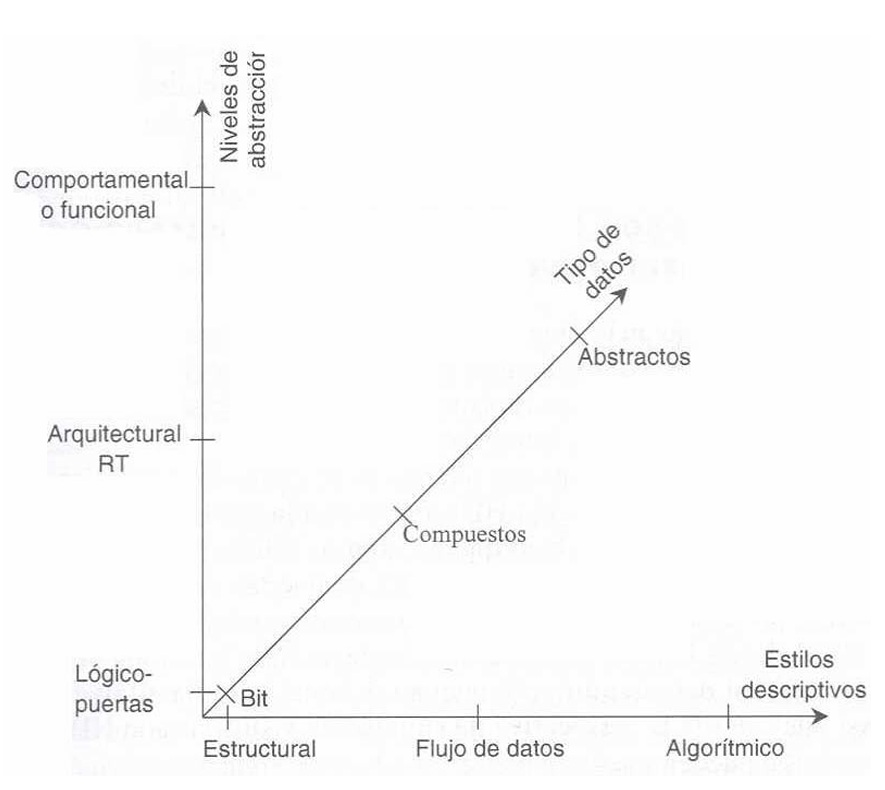
\includegraphics[width=0.5\textwidth, height=6cm]{imagenes/img1} % Reemplaza con el nombre de tu archivo de imagen
    \caption{Niveles de abstracción/precisión y estilos de modelado VHDL.}
    \label{fig:imagen1} % Etiqueta para referenciar la figura
\end{figure} 
%\clearpage

Los lenguajes de descripción de hardware (HDL) fueron desarrollados inicialmente con el propósito de modelar el comportamiento funcional de los componentes electrónicos, permitiendo su simulación previa a la implementación física. No obstante, también son ampliamente utilizados para la descripción estructural de circuitos digitales, facilitando su posterior síntesis y verificación mediante procesos de simulación validados (\ref{fig:imagen2}).
\begin{figure}[h!] % [h!] Fuerza a LaTeX a poner la figura aquí
    \centering % Centra la imagen
     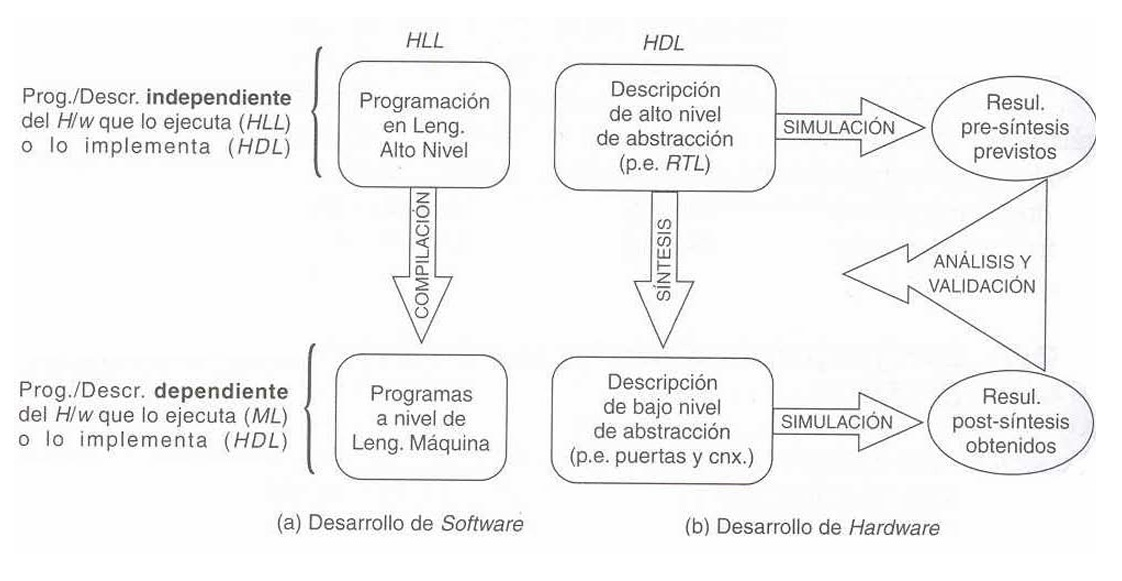
\includegraphics[width=0.8\textwidth, height=6cm]{imagenes/img2} % Reemplaza con el nombre de tu archivo de imagen
    \caption{Desarrollo en software versus hardware: (a) niveles de abstracción y lenguajes de alto nivel y (b) esquema básico del diseño descendente con HDL.  .}
    \label{fig:imagen2} % Etiqueta para referenciar la figura
\end{figure} 

A partir de las descripciones iniciales, los enfoques de diseño descendente (top-down) permiten aplicar procesos progresivos de síntesis que conducen gradualmente a niveles más detallados de implementación, hasta alcanzar una descripción física específica y dependiente de la tecnología utilizada. La validación en cada etapa del diseño se lleva a cabo mediante simulaciones y análisis funcionales, permitiendo iteraciones sucesivas de verificación y corrección hasta lograr un comportamiento conforme a los requisitos especificados ( \ref{fig:imagen2}(b)).


\section{Descripción de la tarjeta de desarollo Altera DE2-115 }

La tarjeta Altera DE2-115, desarrollada por Terasic Technologies, es una plataforma de prototipado basada en la FPGA Cyclone IV EP4CE115F29C7N de Altera (ahora Intel), orientada a entornos educativos, de investigación y desarrollo de sistemas digitales avanzados. Esta tarjeta ofrece una arquitectura versátil que permite implementar desde diseños lógicos básicos hasta sistemas digitales complejos, incluyendo sistemas embebidos, controladores personalizados, procesamiento de señales digitales (DSP) y prototipos de SoC (System-on-Chip).

Entre sus características principales se destaca la presencia de 114,480 elementos lógicos (LEs), 3.888 Kbits de memoria RAM embebida, y 528 pines de entrada/salida de propósito general (GPIO), lo que proporciona una gran flexibilidad para interactuar con múltiples dispositivos periféricos. La tarjeta también incluye memorias externas como SDRAM de 128 MB, SRAM de 2 MB, y Flash NOR de 2 MB, además de soporte para almacenamiento mediante tarjeta SD.

La DE2-115 incorpora interfaces esenciales para el desarrollo de sistemas interactivos, tales como puertos USB, Ethernet Gigabit, salida VGA, entradas y salidas de audio, además de un conjunto de dispositivos de entrada/salida integrados como interruptores, botones, LEDs y displays de siete segmentos. Adicionalmente, cuenta con un oscilador de cristal de 50 MHz y conectores de expansión compatibles con módulos adicionales.

Esta plataforma es ampliamente utilizada en laboratorios académicos y en entornos de investigación aplicada debido a su compatibilidad con herramientas de desarrollo como Quartus Prime, facilitando la implementación de diseños en lenguajes HDL como VHDL y SystemVerilog. Su capacidad para realizar simulación, verificación y síntesis de diseños en una sola herramienta la hace ideal para proyectos de educación superior en ingeniería electrónica, mecatrónica y sistemas digitales. 

Características técnicas destacadas:

FPGA: Altera Cyclone IV EP4CE115F29C7N con 114,480 elementos lógicos (LEs)

\begin{itemize}
	\item Memoria:
		\begin{itemize}
			\item 2 MB SRAM
			\item 128 MB SDRAM
			\item 2 MB Flash NOR
			\item Tarjeta SD para almacenamiento externo
		\end{itemize}
	\item Interfaces de usuario:
		\begin{itemize}
			\item 18 interruptores (switches) y 18 botones pulsadores
			\item 18 LEDs rojos y 9 LEDs verdes
			\item 8 displays de 7 segmentos
		\end{itemize}
	\item Conectividad:
		\begin{itemize}
			\item Puertos USB tipo A y B
			\item Puerto Ethernet 10/100/1000 Mbps (Gigabit)
			\item Entrada/salida VGA
			\item Conectores de expansión GPIO de 40 pines
		\end{itemize}
	\item Audio y Video:
		\begin{itemize}
			\item Entrada y salida de audio (jack de 3.5 mm)
			\item Entrada de señal VGA (con ADC) y salida VGA
		\end{itemize}
	\item Reloj: oscilador de cristal de 50 MHz
	\item Programación y depuración: Soporte JTAG, compatible con Quartus II
\end{itemize}
 
\begin{figure}[h!] % [h!] Fuerza a LaTeX a poner la figura aquí
    \centering % Centra la imagen
     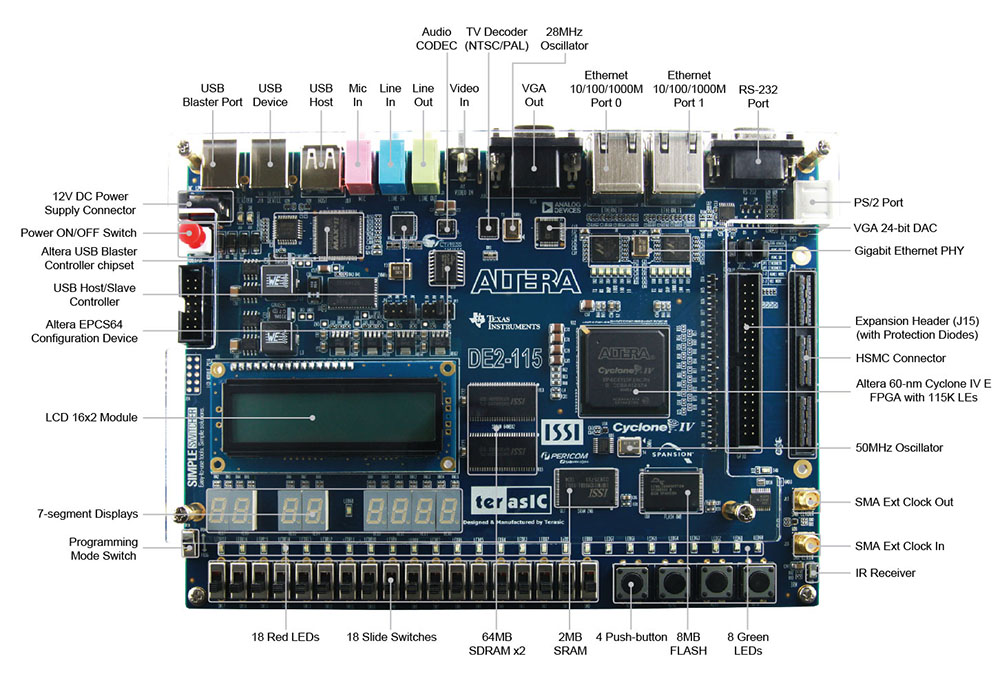
\includegraphics[width=1\textwidth, height=13cm]{imagenes/img3} % Reemplaza con el nombre de tu archivo de imagen
    \caption{Tarjeta de desarollo Altera DE2-115.}
    \label{fig:imagen3} % Etiqueta para referenciar la figura
\end{figure}

%\clearpage


\chapter{Diseño de Plataforma para Transmisión Serial de Datos}

\section{Plataforma de Comunicación Serial para el Cifrado y Descifrado }
La seguridad de la información, especialmente en lo que respecta a la confidencialidad, representa una de las principales preocupaciones en el ámbito de las comunicaciones. Para mitigar los riesgos de acceso no autorizado, es común la implementación de algoritmos criptográficos que aseguren que solo el receptor legítimo pueda interpretar los datos transmitidos.

Uno de los principales objetivos de este trabajo es desarrollar una plataforma basada en FPGA que permita integrar mecanismos de codificación de flujo para proteger la transmisión de datos entre dos dispositivos que se comunican mediante el protocolo UART. En lugar de utilizar UART en su forma tradicional, este protocolo es modificado y ampliado para incorporar una capa de seguridad directamente a nivel de hardware, mejorando así la confidencialidad de la información transmitida.

Para ello, se diseñó una plataforma base que incluye los módulos necesarios para enviar y recibir datos, realizar la codificación y decodificación de los mensajes, y establecer la comunicación segura entre ambos extremos. Esta arquitectura ha sido planteada de forma flexible, permitiendo que el proceso de codificación se defina de manera genérica. De este modo, es posible integrar diferentes algoritmos criptográficos sin necesidad de rediseñar por completo el sistema, lo que facilita su adaptación a distintos niveles de seguridad o aplicaciones específicas.

Un aspecto fundamental para el desempeño de un codificador de flujo es que su velocidad de operación no afecte la eficiencia de la comunicación. Por esta razón, la plataforma está implementada en una FPGA, lo que permite ampliar y modificar el protocolo de comunicación para incluir una capa de seguridad directamente a nivel hardware. Así, el proceso de cifrado se realiza en tiempo real, garantizando que la protección de los datos no genere retrasos ni impacte negativamente en la velocidad de transmisión.

Se realiza la prueba y validación del desempeño de la plataforma mediante la comparación de su funcionamiento al implementar un protocolo personalizado de comunicacion para incrementar el grado de seguridad.

\section{Protocolo Seguro para Comunicación Serial}
Como parte del desarrollo de esta tesis, se aborda el diseño de un sistema de comunicación seguro, iniciando con el análisis de las características fundamentales de los sistemas de comunicación digital y los mecanismos para garantizar que la información transmitida sea recibida y correctamente interpretada únicamente por el destinatario autorizado. Durante este proceso analítico se identifican múltiples criterios que definen las propiedades esenciales para un algoritmo criptográfico eficiente, los cuales serán abordados detalladamente en este capítulo.

En el proceso de establecer los parámetros para una comunicación segura, se busca lograr este objetivo minimizando el impacto sobre los sistemas de comunicación existentes. Cualquier mecanismo implementado para garantizar la seguridad debe ser transparente para el usuario y operar en tiempo real, sin afectar las características esenciales de la comunicación, tales como la calidad y la velocidad de transmisión.

Actualmente, la mayoría de los sistemas de comunicación emplean transmisión de datos serial, generalmente en modo full-duplex, para el intercambio de información. En la búsqueda de sistemas de comunicación seguros, funcionales y eficientes, es necesario analizar y evaluar en tiempo real la ejecución de un algoritmo criptográfico estándar. Posteriormente, será posible implementar y evaluar otros algoritmos conforme a las necesidades del sistema.

A partir de los lineamientos previamente establecidos, se definen las características fundamentales para el diseño de la plataforma de comunicación criptográfica, las cuales son:



\begin{enumerate}
\renewcommand{\theenumi}{\alph{enumi}}
\renewcommand{\labelenumi}{{\theenumi})}
\item Integración transparente: El sistema de cifrado debe ser incorporado en la línea de comunicación sin necesidad de modificar el equipo de comunicaciones existente, manteniendo así la compatibilidad con la infraestructura actual.

\item Compatibilidad con comunicación serial full-duplex asíncrona: La plataforma debe ser capaz de manejar flujos de datos bidireccionales simultáneos (full-duplex) en modo asíncrono, soportando múltiples velocidades de transmisión comúnmente utilizadas en entornos industriales o embebidos.

\item Flexibilidad criptográfica: Debe ofrecer la posibilidad de cambiar el algoritmo de cifrado de manera sencilla, permitiendo al usuario seleccionar entre distintas opciones según los requerimientos de seguridad del sistema.

\item Procesamiento en tiempo real: Las operaciones de cifrado y descifrado deben ejecutarse de forma continua y en tiempo real, sin interrupciones en el flujo de información, garantizando la integridad y la eficiencia de la comunicación.
\end{enumerate} 

Para alcanzar el primer objetivo —la integración transparente del sistema de seguridad— se diseñaron módulos hardware que pueden ser instalados en ambos extremos de la línea de comunicación. Estos dispositivos pueden colocarse directamente en los puntos finales del canal de transmisión, o bien actuar como una interfaz entre el usuario y el equipo de comunicación. La ubicación óptima dependerá del contexto de uso, de las características del equipo involucrado y del medio físico de transmisión utilizado.

La Figura (\ref{fig:imagen4}) muestra un diagrama de bloques que ilustra cómo puede integrarse el sistema de seguridad dentro de una arquitectura de comunicación serial, permitiendo el cifrado de los datos sin alterar la funcionalidad básica del canal.

\begin{figure}[h!] % [h!] Fuerza a LaTeX a poner la figura aquí
    \centering % Centra la imagen
     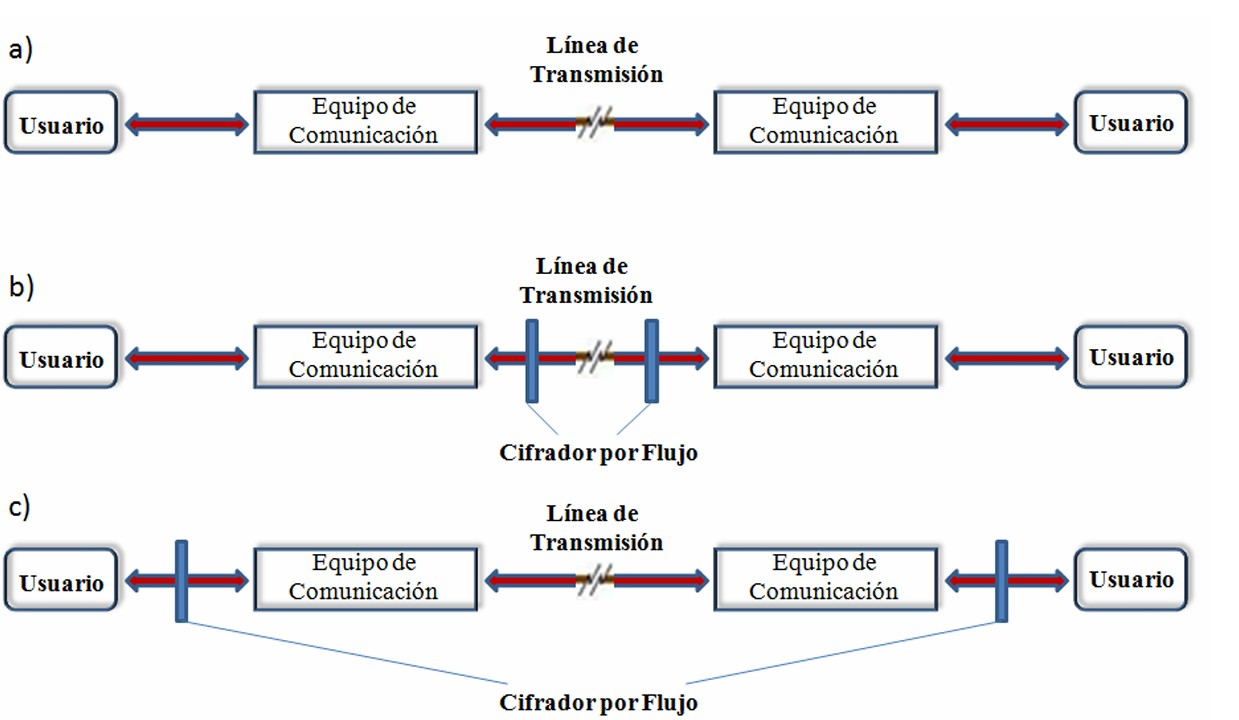
\includegraphics[width=1\textwidth, height=8cm]{imagenes/img4} % Reemplaza con el nombre de tu archivo de imagen
    \caption{Diagrama de bloques de un sistema de comunicación simplificado. a) Sistema Inseguro. 
b) Sistema con el cifrado en los extremos de la línea de la transmisión. c) Sistema con el cifrado 
como interfaz entre el usuario y el  equipo de comunicación. }
    \label{fig:imagen4} % Etiqueta para referenciar la figura
\end{figure} 

El mecanismo encargado del cifrado debe incluir, en términos generales, un módulo central de control responsable de coordinar todo el proceso de cifrado y descifrado. Este módulo gestiona el flujo de datos entre dos interfaces de comunicación serial, actuando como intermediario entre el transmisor y el receptor. Su funcionamiento se basa en controlar la entrada y salida de datos cifrados y descifrados de acuerdo con la lógica definida por el algoritmo criptográfico. La Figura (\ref{fig:imagen5}) ilustra la estructura general del sistema, destacando el papel del controlador central dentro del esquema de comunicación segura.

\clearpage

\begin{figure}[h!] % [h!] Fuerza a LaTeX a poner la figura aquí
    \centering % Centra la imagen
     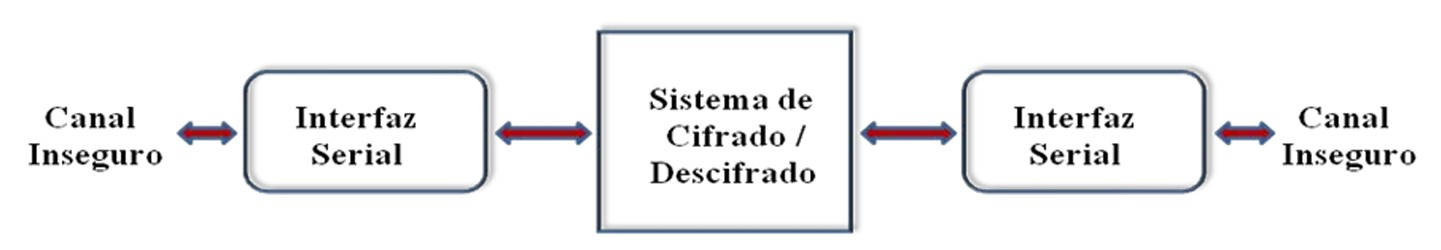
\includegraphics[width=0.8\textwidth, height=3cm]{imagenes/img5} % Reemplaza con el nombre de tu archivo de imagen
    \caption{Diagrama de bloques del dispositivo de cifrado y Descifrado.}
    \label{fig:imagen5} % Etiqueta para referenciar la figura
\end{figure} 

Con el objetivo de garantizar que el proceso de cifrado y descifrado se ejecute de forma continua, sin interrumpir ni degradar el flujo original de información, se opta por el uso de algoritmos de cifrado por flujo. Este tipo de algoritmos permite el procesamiento de los datos en tiempo real, bit a bit o byte a byte, lo cual es especialmente adecuado para sistemas de comunicación serial donde la información se transmite de manera secuencial.

\section{Diseño de la Plataforma Criptográfica}

Para llevar a cabo el diseño de la plataforma criptográfica, se parte de las especificaciones definidas en la sección anterior. El método comúnmente empleado para el intercambio de información es la transmisión de datos en serie. Por ello, se implementan dos puertos “Universal Asynchronous Receiver/Transmitter” (UART), los cuales permiten la conexión de la plataforma con el medio de comunicación: uno destinado a recibir y enviar datos en su formato original hacia y desde el usuario, y otro encargado de manejar la información cifrada a través del canal de transmisión. Esta configuración facilita la incorporación del proceso de cifrado en cualquier sistema de comunicación digital que utilice transmisión serial full-dúplex asincrónica, requiriendo únicamente el desarrollo de una interfaz adecuada según el punto de integración dentro del sistema.

Por otro lado para poner la plataforma criptográfica en ejecución se decide utilizar un FPGA, aprovechando sus características, incluyendo su operación de alta velocidad, bajo costo, facilidad de empleo y reconfiguración. En trabajo se decidió utilizar una tarjeta de desarrollo con un EP4CE115integrado, de la familia a Cyclone® IVSpartan. Este FPGA es de tamaño medio, con el equivalente a 114,480 mil compuertas lógicas. El integrado tiene gran capacidad de poder integrar la plataforma criptográfica junto con cualquier bloque que se quiera cifrar y evaluar. Esta plataforma de desarrollo funciona a 50 [MHz], que permite configurar el UART para funcionar a una velocidad de 3.125 [Mbps], que es bastante para funcionar en tiempo real como la mayor parte de los sistemas de comunicación.

Ahora bien para probar la operación total del cifrador, que podría ser integrado en una línea de comunicación, primero se desarrolló el esquema de cifrado que se muestra en la Figura (\ref{fig:imagen6}). Esta implementación consiste de un módulo con una máquina de estados que controle al dispositivo, maneje la operación de los UART y que lleve a cabo los procesos de cifrado y descifrado. 

\begin{figure}[h!] % [h!] Fuerza a LaTeX a poner la figura aquí
    \centering % Centra la imagen
     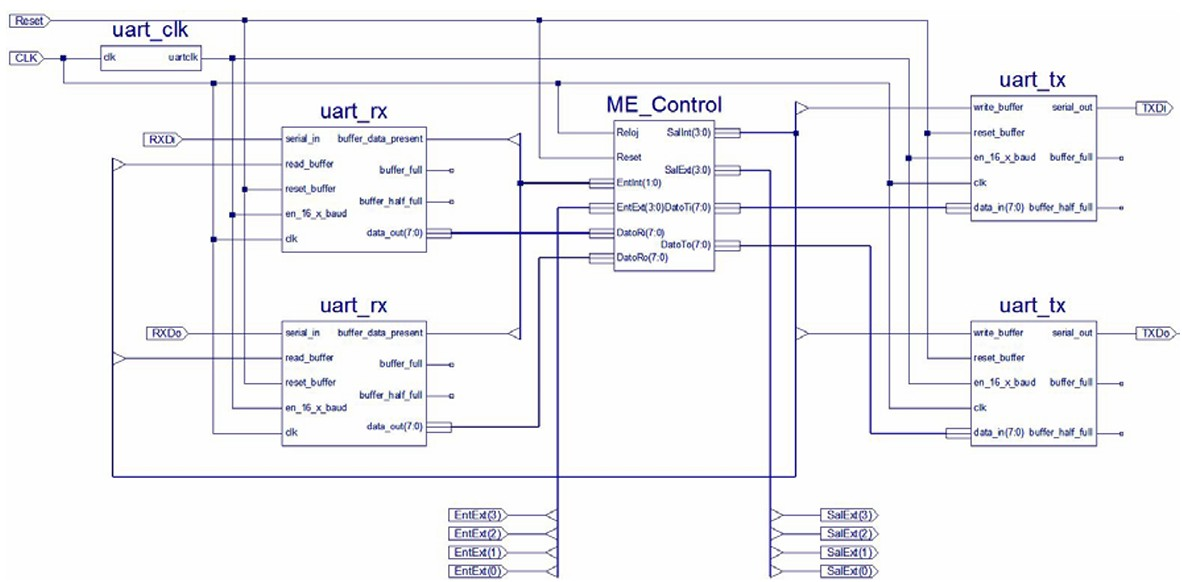
\includegraphics[width=0.9\textwidth, height=8cm]{imagenes/img6} % Reemplaza con el nombre de tu archivo de imagen
    \caption{Diseño de la Plataforma integrando el proceso de cifrado y el bloque de control.}
    \label{fig:imagen6} % Etiqueta para referenciar la figura
\end{figure} 

Este dispositivo se emplea para validar el funcionamiento de la plataforma criptográfica, permitiendo la ejecución del proceso de cifrado dentro de un sistema de comunicación. Durante las pruebas experimentales, se utilizaron dos de estos dispositivos conectados entre dos computadoras que se comunicaban mediante un puerto serial RS-232. Los resultados obtenidos a partir de estas pruebas se detallan en el capítulo \#\#\#\#, correspondiente a los resultados.

Con este diseño se logra verificar el funcionamiento general de la plataforma criptográfica; sin embargo, no se satisfacen completamente los requisitos establecidos, particularmente en lo referente a la flexibilidad para cambiar el algoritmo de cifrado. Esto se debe a que el módulo criptográfico está integrado dentro de la máquina de estados del bloque de control, lo que implica que incluso un cambio simple en el algoritmo requiere modificaciones estructurales en todo el sistema.

Para solucionar esta limitación, se propone una reestructuración del diseño, separando el elemento de seguridad del bloque de control. Así, los procesos de cifrado y descifrado se implementan en un módulo independiente, permitiendo que el bloque de control se limite exclusivamente a gestionar la comunicación a través de los UARTs, una vez que los datos han sido procesados por el bloque criptográfico.

Se tiene especial cuidado en proporcionar al bloque de cifrado/descifrado una interfaz genérica que le permita interactuar con el bloque de control sin depender del algoritmo utilizado. Para ello, se define un protocolo simple de handshake que permite al bloque de cifrado/descifrado recibir una señal cuando hay datos listos para ser procesados, y notificar al bloque de control una vez finalizado el procesamiento. Este mecanismo asegura que no se pierda información, evitando que se envíen nuevos datos al cifrador antes de que haya finalizado el procesamiento de los datos actuales.

Si bien el alcance de esta tesis se limita a la implementación del algoritmo de cifrado CESAR dentro de la plataforma de comunicación, el diseño apunta a una arquitectura escalable que permita integrar distintos algoritmos criptográficos. De esta manera, cuando se requiera implementar un nuevo dispositivo de cifrado/descifrado, bastará con desarrollar el bloque correspondiente al nuevo algoritmo y conectarlo a la plataforma para obtener un sistema completamente funcional. El dispositivo resultante puede observarse en la Figura (\ref{fig:imagen7}).

\begin{figure}[h!] % [h!] Fuerza a LaTeX a poner la figura aquí
    \centering % Centra la imagen
     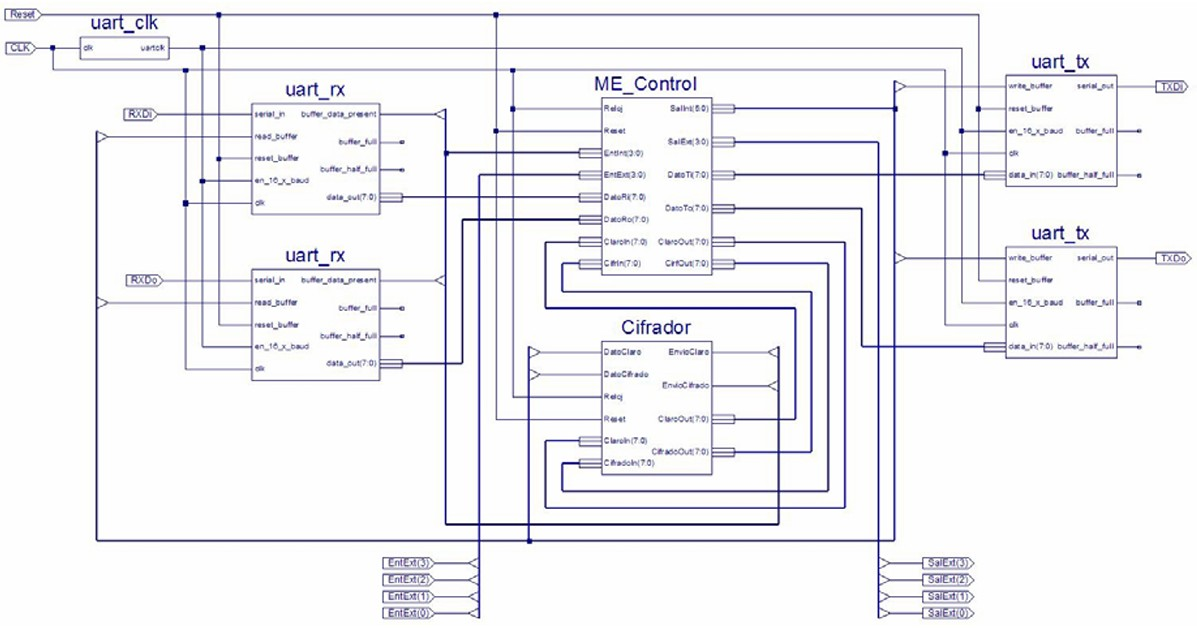
\includegraphics[width=1\textwidth, height=8cm]{imagenes/img7} % Reemplaza con el nombre de tu archivo de imagen
    \caption{ Diseño de la Plataforma Criptográfica incorporando el proceso de cifrado/descifrado 
como un bloque independiente.}
    \label{fig:imagen7} % Etiqueta para referenciar la figura
\end{figure} 


\clearpage

\section{Aspectos Clave del UART}

La unidad UART se encarga de controlar los puertos y dispositivos serie destinados a la comunicación de datos. En la tarjeta de desarrollo Altera DE2-115 se encuentra implementado un puerto RS-232; sin embargo, este no fue utilizado en el presente diseño. En su lugar, se optó por la personalización de los pines de comunicación a través del Expansion Header (J15), con el propósito de facilitar la integración práctica del sistema, tal como se ilustra en la Figura (\ref{fig:imagen3}). Se desarrollaron los bloques necesarios para generar el módulo encargado de implementar una UART personalizada en lenguaje Verilog, destinada a los pines correspondientes del Expansion Header.

En el contexto del diseño digital mediante RTL sobre FPGA, la Unidad de Recepción-Transmisión Asíncrona (UART) cumple funciones esenciales, entre las que destacan la gestión de interrupciones provenientes de los dispositivos conectados al puerto serie y la conversión de datos entre los formatos paralelo y serie. En este proceso, los datos en formato paralelo provenientes del bus del sistema son transformados a formato serie para su transmisión a través de la interfaz de comunicación, mientras que los datos recibidos en formato serie son convertidos nuevamente a formato paralelo para su procesamiento interno.

\subsection{Propiedades Principales del UART}

Para fines demostrativos del proceso de cifrado y con el objetivo de verificar la correcta transmisión de la información, se implementó la comunicación estándar hacia computadoras personales. Es importante señalar que no es posible establecer una comunicación directa entre la tarjeta de desarrollo Altera DE2-115 y un ordenador, debido a que uno de los objetivos de este trabajo consistió en modificar el protocolo UART para incorporar una capa adicional de seguridad a nivel de hardware. En este sentido, si la tarjeta se conecta directamente a un ordenador, este únicamente dispondrá de la comunicación bajo el estándar UART original, lo que imposibilita una transmisión exitosa entre ambas plataformas (PC y FPGA). Para solventar esta limitación, se empleó una segunda FPGA del mismo modelo (Altera DE2-115), en la cual se implementó la misma arquitectura. De esta forma, la comunicación entre ambas FPGA resulta exitosa y adecuada, considerando que en una aplicación real no se requerirá del uso de ordenadores para el monitoreo de la información.


\section{Principio de Operación de la UART}
En investigaciones previas se han propuesto mecanismos de seguridad sobre UART, pero en su mayoría dependen de software, lo que limita la eficiencia y vulnerabilidad ante ataques. Otros estudios han demostrado que la implementación de algoritmos criptográficos en FPGA, como AES en modo CTR, es factible y efectiva para mejorar la seguridad sin afectar el rendimiento significativamente.

\subsection{Mecanismo de transmisión y recepción UART}

Un UART, debido a la forma en que están construidos el transmisor y el receptor, no opera de manera sincronizada; sin embargo, ambos emplean un tiempo de referencia con cierta tolerancia que permite la transferencia serial de cada byte de datos. La transmisión se realiza de forma serial, enviando primero el bit menos significativo (LSB) a una razón de bits determinada (tasa en baud), la cual es conocida tanto por el transmisor como por el receptor. De esta manera, el transmisor puede iniciar el envío de datos en cualquier momento, mientras que el receptor requiere un mecanismo que le permita identificar cuándo ha sido transmitido el primer bit (LSB). Este proceso se logra mediante el envío de una señal de inicio (start bit), activada en nivel bajo durante la duración de un bit, como se muestra en la Figura (\ref{fig:imagen8}).

\begin{figure}[h!] % [h!] Fuerza a LaTeX a poner la figura aquí
    \centering % Centra la imagen
     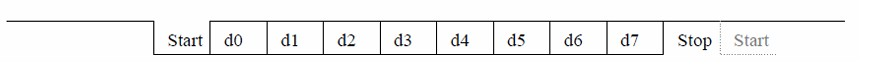
\includegraphics[width=0.8\textwidth, height=1.5cm]{imagenes/img8} % Reemplaza con el nombre de tu archivo de imagen
    \caption{ Esquema de tiempo para la transmisión de un byte.}
    \label{fig:imagen8} % Etiqueta para referenciar la figura
\end{figure} 

El receptor utiliza el flanco de bajada del bit de inicio para activar un circuito de temporización interno. Este tiempo de referencia permite muestrear la señal de entrada serial aproximadamente a la mitad de la duración de cada bit de datos, momento en el que se espera que el valor del bit sea estable. Una vez que se ha leído el último bit de datos (MSB), el receptor verifica que el bit de parada esté en nivel alto, como se espera, lo cual confirma que la operación de recepción se realizó correctamente Figura (\ref{fig:imagen9}).

\begin{figure}[h!] % [h!] Fuerza a LaTeX a poner la figura aquí
    \centering % Centra la imagen
     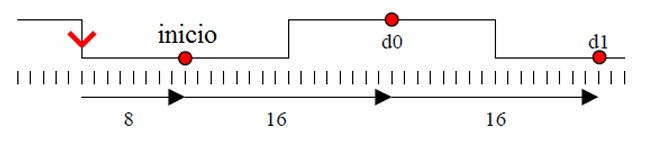
\includegraphics[width=0.7\textwidth, height=1.8cm]{imagenes/img9} % Reemplaza con el nombre de tu archivo de imagen
    \caption{  Esquema temporal para la recepción de datos.}
    \label{fig:imagen9} % Etiqueta para referenciar la figura
\end{figure} 

El receptor se vuelve a sincronizar utilizando el flanco de bajada de cada bit de inicio mediante su circuito temporal interno. Para que la transmisión y recepción funcionen correctamente, el tiempo de ambos sistemas solo necesita coincidir dentro de una tolerancia de aproximadamente la mitad del período de un bit en cada 10 períodos de bit. Esta precisión del 5\% es difícil de alcanzar con sistemas digitales convencionales.

Al igual que muchas implementaciones UART, estos macros esperan un tiempo de referencia proporcionado mediante una señal habilitadora, denominada ''en\_16\_x\_baud'', que se aplica a razón de una vez por cada 16 bits transmitidos.


\subsection{Criterios para la terminación de la transmisión UART}

En condiciones normales, una línea serial se mantiene activa en nivel alto, de modo que un nuevo bit de inicio se identifica mediante un flanco de bajada. Sin embargo, bajo una condición de fallo, el transmisor puede mantener continuamente la línea en nivel bajo (por ejemplo, por falta de alimentación). En este caso, el receptor interpretará el nivel bajo como un bit de inicio seguido de bits de datos en cero. Como consecuencia, el bit de parada no será válido y la trama incorrecta será descartada, Figura (\ref{fig:imagen10}).

\begin{figure}[h!] % [h!] Fuerza a LaTeX a poner la figura aquí
    \centering % Centra la imagen
     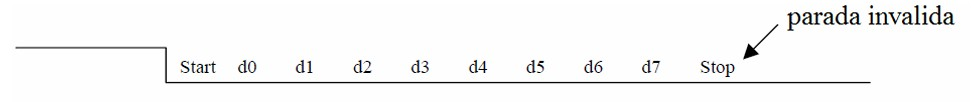
\includegraphics[width=0.9\textwidth, height=1.5cm]{imagenes/img10} % Reemplaza con el nombre de tu archivo de imagen
    \caption{  Esquema temporal de una parada invalida.}
    \label{fig:imagen10} % Etiqueta para referenciar la figura
\end{figure} 

El receptor permanecerá a la espera hasta que la línea vuelva a nivel alto y únicamente se volverá a sincronizar con el siguiente flanco de bajada correspondiente al bit de inicio Figura \ref{fig:imagen11}).

\begin{figure}[h!] % [h!] Fuerza a LaTeX a poner la figura aquí
    \centering % Centra la imagen
     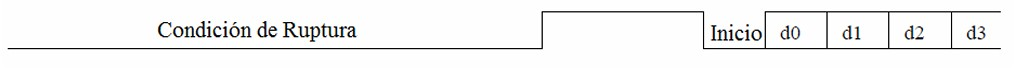
\includegraphics[width=0.8\textwidth, height=1.4cm]{imagenes/img11} % Reemplaza con el nombre de tu archivo de imagen
    \caption{  Esquema temporal de una operacion de ruptura.}
    \label{fig:imagen11} % Etiqueta para referenciar la figura
\end{figure} 

El macro del transmisor, de forma natural, no realizará ninguna transmisión bajo una condición de fallo. En cambio, el macro del receptor reconoce esta situación y continúa operando según lo descrito previamente.

\subsection{Tasa de baudios de la UART}

A partir de los macros de transmisión y recepción se generan los tiempos de la señal de referencia ''en\_16\_x\_baud''. Como indica su nombre, esta señal debe aplicarse al macro de la tasa de transmisión, que opera a 16 veces la velocidad de bits deseada Figura (\ref{fig:imagen12}).

\begin{figure}[h!] % [h!] Fuerza a LaTeX a poner la figura aquí
    \centering % Centra la imagen
     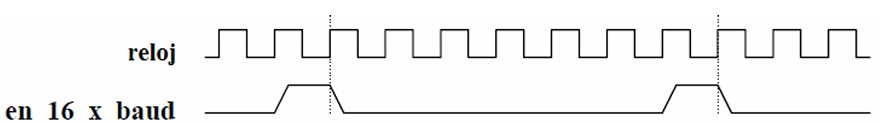
\includegraphics[width=0.8\textwidth, height=1.4cm]{imagenes/img12} % Reemplaza con el nombre de tu archivo de imagen
    \caption{  Esquema temporal en BAUD's.}
    \label{fig:imagen12} % Etiqueta para referenciar la figura
\end{figure} 

De esta forma, la señal se utiliza como un reloj habilitador dentro de los macros. Debe ser generada a partir de un reloj sincronizado y tener una duración de pulso equivalente a un solo ciclo de reloj (lo que requiere, al menos, una frecuencia de reloj máxima dividida entre 16).

\subsection{Implementación RTL del Bloque UART\_Tx y UART\_rx }
El UART receptor está formado por un archivo en Verilog. El nombre del archivo es ''receiver.sv'' que esta implementando en combinación con los modulos de ''binary\_to\_7seg.sv'' y ''transmitter.sv'', los modulos tanto de receiver y transmitter cuentan con su capa de cifrado y descifrado, incluyendo las variantes de rotación de bits y la selecció de rango de esta misma.

\subsection{Configuración de las Interfaces Seriales con las TarjetasAltera DE2–115 }

En la Figura (\ref{fig:imagen13}) se observa la conexión de los puertos definidos por el usuario, lo cual pone de manifiesto la flexibilidad inherente a las FPGA. Esta característica permite que los pines de entrada y salida no estén restringidos a conectores predeterminados, sino que puedan ser asignados libremente por el diseñador. De esta manera, además de optimizar la arquitectura del sistema, se incrementa la dificultad para que un agente externo pueda identificar los pines específicos donde se lleva a cabo la comunicación (Brown \& Vranesic, 2013).

\begin{figure}[h!] % [h!] Fuerza a LaTeX a poner la figura aquí
    \centering % Centra la imagen
     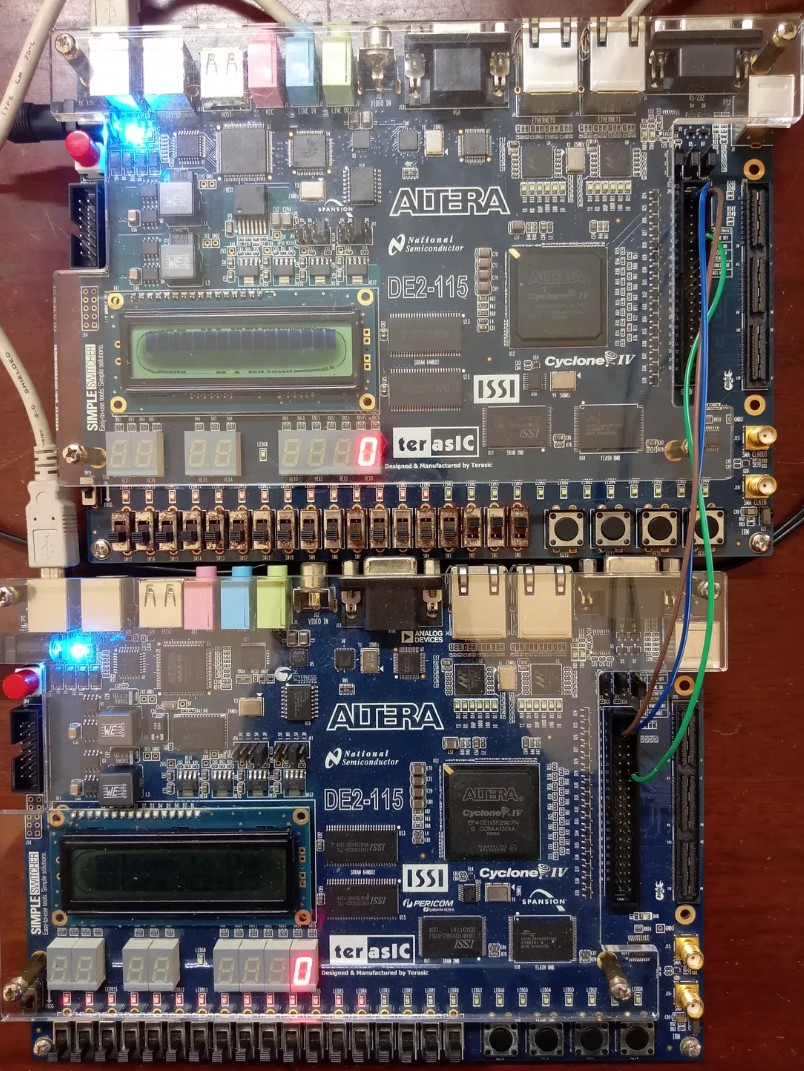
\includegraphics[width=1\textwidth, height=12cm]{imagenes/img13} % Reemplaza con el nombre de tu archivo de imagen
    \caption{  Conexion de las dos plataformas Altera DE2–115 mediante la selección de pines del modulo Jtag .}
    \label{fig:imagen13} % Etiqueta para referenciar la figura
\end{figure} 

\clearpage
En la Figura (\ref{fig:imagen14}) se ilustra la definición de los pines destinados a la comunicación serial, la cual fue realizada dentro del software Quartus. Este procedimiento permite establecer de manera explícita las asignaciones físicas entre los pines de la FPGA y las señales lógicas del diseño, asegurando así la correcta implementación del sistema en el dispositivo reconfigurable. 

\begin{figure}[h!] % [h!] Fuerza a LaTeX a poner la figura aquí
    \centering % Centra la imagen
     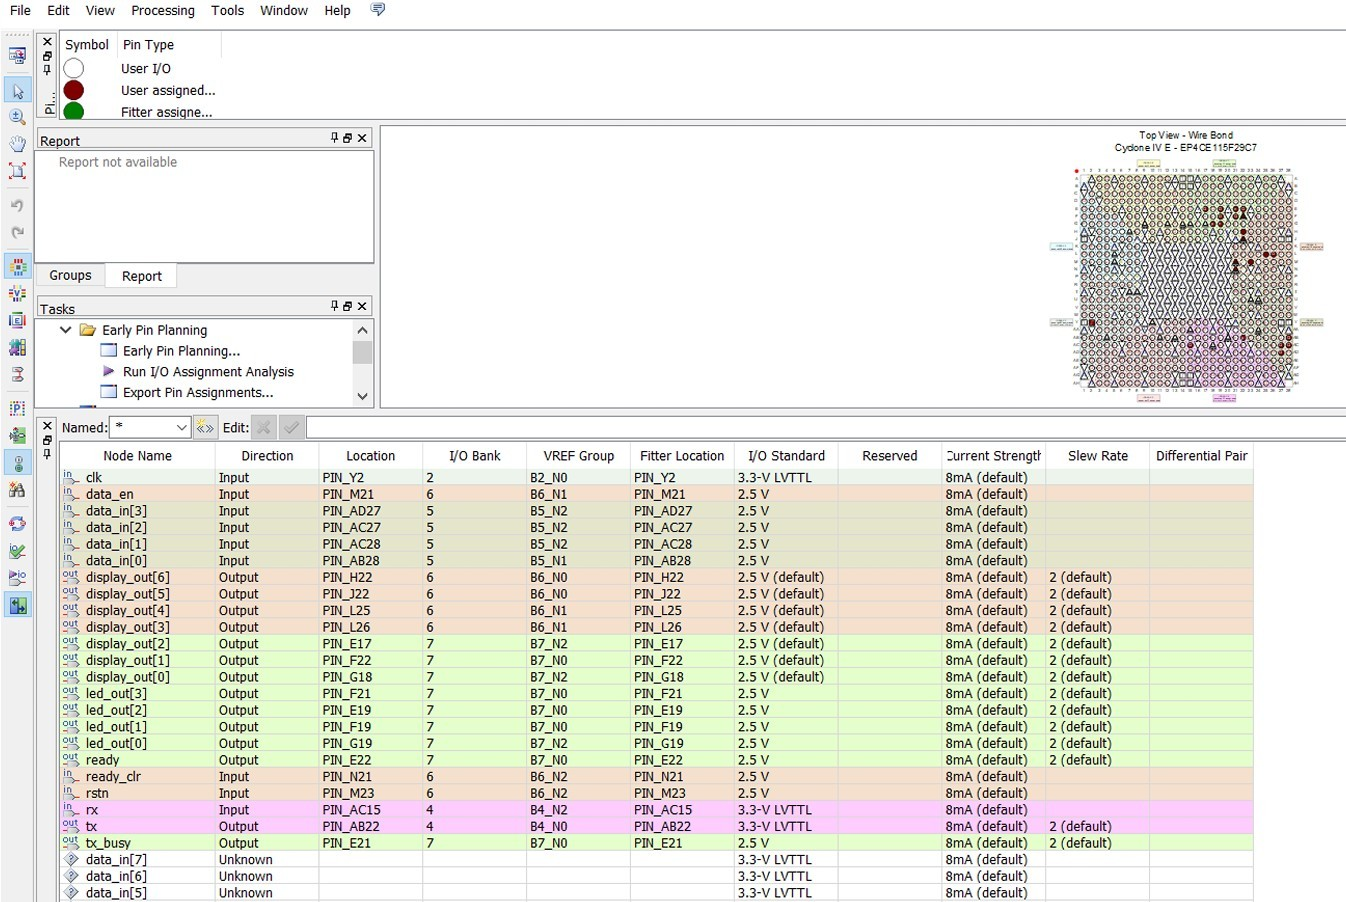
\includegraphics[width=1\textwidth, height=10cm]{imagenes/img14} % Reemplaza con el nombre de tu archivo de imagen
    \caption{  Seleccion de pines mediante el Software Quartus.}
    \label{fig:imagen14} % Etiqueta para referenciar la figura
\end{figure} 

\clearpage
A continuación, en la Figura (\ref{fig:imagen15}), se presenta el esquema de las conexiones empleadas para la validación del sistema. Con el propósito de verificar el correcto funcionamiento de los módulos implementados, se estableció una comunicación entre dos ordenadores conectados en los extremos, lo que permitió comprobar la transmisión y recepción adecuada de los datos.

\begin{figure}[h!] % [h!] Fuerza a LaTeX a poner la figura aquí
    \centering % Centra la imagen
     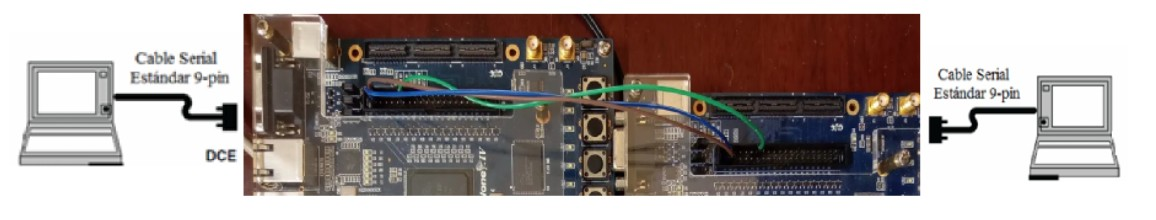
\includegraphics[width=1\textwidth, height=3cm]{imagenes/img15} % Reemplaza con el nombre de tu archivo de imagen
    \caption{ Esquema de conexiones para la plataforma de cifrado y su validación.}
    \label{fig:imagen15} % Etiqueta para referenciar la figura
\end{figure} 

\chapter{RESULTADOS}

\section{Resultados}

En este último capítulo se presentan los resultados obtenidos durante el desarrollo de las implementaciones propuestas, tanto en relación con los objetivos particulares como con el objetivo general de la presente tesis. Algunos de estos resultados se contrastan con los publicados en los estándares correspondientes, tanto para el algoritmo de cifrado seleccionado y programado, como para el modo de operación implementado. Asimismo, se incluyen resultados derivados de la aplicación desarrollada para la integración de los mecanismos de seguridad, específicamente aquellos vinculados a las pruebas realizadas en la plataforma criptográfica destinada a la comunicación serial segura. Finalmente, para la consulta de los códigos fuente y ciertos detalles específicos de la programación, el lector puede remitirse a los anexos ubicados al final de este capítulo.

Con el fin de validar el mecanismo de ofuscación propuesto como una mejora al cifrado César tradicional, se llevaron a cabo una serie de experimentos tanto en el ámbito de software como en el de hardware. El objetivo principal fue demostrar que la integración de una capa adicional de ofuscación no solo incrementa la complejidad del proceso de descifrado del mensaje encriptado, sino que también preserva la equivalencia funcional entre el prototipo en software y su implementación en hardware.

La primera etapa de la experimentación consistió en el desarrollo de un script en Python que implementaba el cifrado César combinado con la técnica de ofuscación propuesta. Este entorno permitió un prototipado rápido y la verificación de la corrección funcional. Se utilizaron diversos conjuntos de datos de entrada, incluyendo cadenas alfanuméricas y secuencias binarias, los cuales fueron sometidos a pruebas de cifrado y descifrado. Posteriormente, se aplicaron medidas estadísticas para evaluar la distribución de los caracteres del texto cifrado  Figura (\ref{fig:imagen16}, con el objetivo de confirmar que la ofuscación lograba una reducción en los patrones de frecuencia predecibles, típicamente explotables en los cifrados clásicos por sustitución. Los gráficos resultantes evidenciaron un aplanamiento notable en las distribuciones de frecuencia de los caracteres, lo que indica que el cifrado modificado mitiga de manera efectiva una de las principales debilidades del esquema César tradicional.


\begin{figure}[h!] % [h!] Fuerza a LaTeX a poner la figura aquí
    \centering % Centra la imagen
     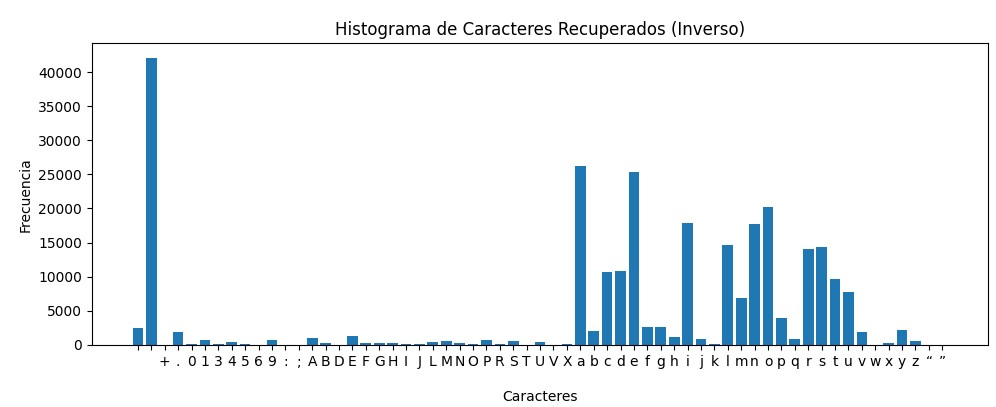
\includegraphics[width=1\textwidth, height=6cm]{imagenes/img16} % Reemplaza con el nombre de tu archivo de imagen
    \caption{ Distribución de texto simple en español.}
    \label{fig:imagen16} % Etiqueta para referenciar la figura
\end{figure} 

Tras la validación exitosa en el dominio de software, el algoritmo fue traducido a una descripción de hardware adecuada para su implementación en FPGA. Específicamente, se diseñó un bloque RTL (Register Transfer Level) utilizando VHDL con el fin de replicar las operaciones tanto del cifrado César como de la capa de ofuscación. La elección de RTL aseguró que el diseño permaneciera sintetizable y pudiera desplegarse físicamente en la plataforma FPGA Altera DE2-115. Este proceso de traducción requirió especial atención al temporizado, la utilización de recursos y la gestión de la concurrencia, ya que la ejecución en hardware introduce restricciones que no están presentes en la ejecución secuencial del software.

La simulación del bloque RTL se llevó a cabo antes de la síntesis, garantizando que la salida coincidiera con la implementación de referencia en Python en todos los vectores de prueba. El análisis de formas de onda confirmó la correcta alineación de las rutas de datos, la sincronización del reloj y el comportamiento de la lógica de control. Posteriormente, el diseño fue sintetizado, colocado y ruteado sobre la FPGA. Los reportes de utilización de recursos indicaron que la lógica adicional de ofuscación introdujo únicamente un incremento moderado en el consumo de elementos lógicos, manteniéndose ampliamente dentro de la capacidad del dispositivo Cyclone IV.
\clearpage
Para validar aún más la efectividad del diseño en hardware, se recolectaron resultados experimentales directamente de la implementación en la FPGA. Secuencias de texto de entrada fueron encriptadas, procesadas a través del mecanismo de ofuscación y posteriormente desencriptadas en tiempo real. Los textos cifrados resultantes fueron nuevamente sometidos a un análisis estadístico de frecuencias (véase Fig. \ref{fig:imagen17}). La comparación entre las distribuciones generadas en software y en hardware confirmó la equivalencia funcional: ambas plataformas alcanzaron niveles similares de dispersión e imprevisibilidad de caracteres.

\begin{figure}[h!] % [h!] Fuerza a LaTeX a poner la figura aquí
    \centering % Centra la imagen
     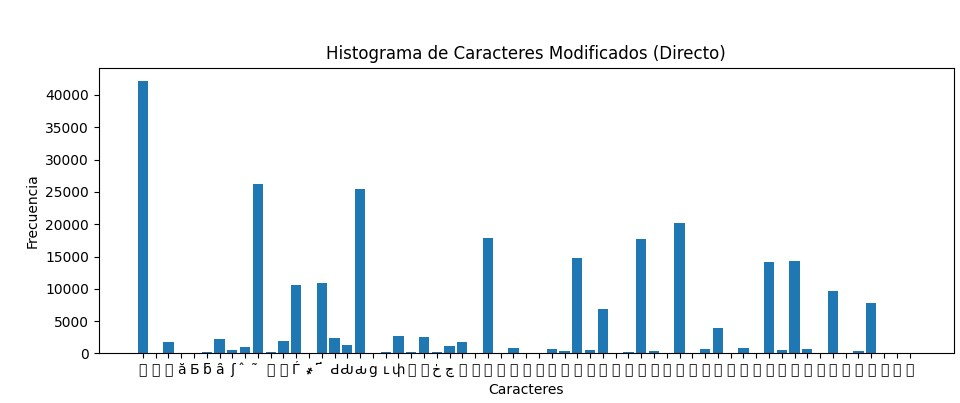
\includegraphics[width=1\textwidth, height=6cm]{imagenes/img17} % Reemplaza con el nombre de tu archivo de imagen
    \caption{ Distribución del texto cifrado producido por la capa de ofuscación implementada en hardware..}
    \label{fig:imagen17} % Etiqueta para referenciar la figura
\end{figure} 

%\newgeometry{margin=1cm,includefoot}
%\layout
%\printinunitsof{cm}
%\pagevalues



%%%%%%fin del archivo
\endinput 